% docs/slides/preamble.tex -- 五份 deck 共享
\documentclass[aspectratio=169,11pt]{beamer}

% ==== 中文与字体 ====
\usepackage[UTF8,fontset=none]{ctex}
\usepackage{fontspec}

\IfFontExistsTF{PingFang SC}{%
  \setCJKmainfont{PingFang SC}[BoldFont=PingFang SC,ItalicFont=PingFang SC,AutoFakeSlant=0.15]
  \setCJKsansfont{PingFang SC}[ItalicFont=PingFang SC,AutoFakeSlant=0.15]
  \setCJKmonofont{PingFang SC}
}{%
  \IfFontExistsTF{Source Han Sans SC}{%
    \setCJKmainfont{Source Han Sans SC}
    \setCJKsansfont{Source Han Sans SC}
  }{%
    \IfFontExistsTF{Noto Sans CJK SC}{%
      \setCJKmainfont{Noto Sans CJK SC}
      \setCJKsansfont{Noto Sans CJK SC}
    }{%
      \setCJKmainfont{Heiti SC}
      \setCJKsansfont{Heiti SC}
    }
  }
}

\IfFontExistsTF{Helvetica Neue}{\setmainfont{Helvetica Neue}}{%
  \IfFontExistsTF{Inter}{\setmainfont{Inter}}{}}
\IfFontExistsTF{JetBrains Mono}{\setmonofont{JetBrains Mono}[Scale=0.85]}%
  {\setmonofont{Menlo}[Scale=0.85]}

% ==== 颜色 ====
\usepackage{xcolor}
\definecolor{cMain}{HTML}{1F4E79}
\definecolor{cAccent}{HTML}{E07A1F}
\definecolor{cGray}{HTML}{595959}
\definecolor{cMute}{HTML}{F4F4F4}
\definecolor{cOK}{HTML}{2E7D32}
\definecolor{cBad}{HTML}{B23A3A}
\definecolor{cWarn}{HTML}{C8A300}

% ==== 主题 ====
\usepackage{tcolorbox}
\usetheme{metropolis}
\metroset{progressbar=frametitle,numbering=fraction,block=fill}
\setbeamercolor{frametitle}{bg=cMain,fg=white}
\setbeamercolor{progress bar}{fg=cAccent,bg=cMute}
\setbeamercolor{alerted text}{fg=cAccent}
\setbeamercolor{title}{fg=cMain}

% metropolis 默认尝试 Fira Sans，未安装时 fallback 到 Latin Modern Sans。
% 这里在主题加载后显式覆盖，强制使用 macOS 上一定存在的 Helvetica Neue，
% 跟中文 PingFang 风格一致；找不到则按顺序尝试 Inter / Arial。
\IfFontExistsTF{Helvetica Neue}{%
  \setsansfont{Helvetica Neue}%
}{%
  \IfFontExistsTF{Inter}{\setsansfont{Inter}}{%
    \IfFontExistsTF{Arial}{\setsansfont{Arial}}{}}%
}

% ==== TikZ ====
\usepackage{tikz}
\usetikzlibrary{positioning,arrows.meta,fit,shapes.geometric,calc,%
  decorations.pathmorphing,backgrounds}

\tikzset{
  node-box/.style={draw=cMain,thick,rounded corners=2pt,
    minimum height=8mm,minimum width=18mm,align=center,font=\small},
  node-state/.style={draw=cMain,thick,circle,minimum size=14mm,
    align=center,font=\small},
  node-ok/.style={draw=cOK,thick,fill=cOK!10},
  node-warn/.style={draw=cWarn,thick,fill=cWarn!15},
  node-bad/.style={draw=cBad,thick,fill=cBad!10},
  % 色盲友好的状态机三态：蓝 (正常/Closed) / 橙 (告警/Open) / 灰 (中间/HalfOpen)
  % 避免 red-green 二元区分，改用 hue + lightness 双通道。
  node-state-normal/.style={draw=cMain,thick,fill=cMain!12},
  node-state-alert/.style={draw=cAccent,thick,fill=cAccent!18},
  node-state-transition/.style={draw=cGray,thick,fill=cGray!18},
  arrow/.style={-{Stealth[length=2mm]},thick,draw=cMain},
  arrow-async/.style={-{Stealth[length=2mm]},thick,dashed,draw=cGray},
  arrow-bad/.style={-{Stealth[length=2mm]},thick,draw=cBad},
  arrow-alert/.style={-{Stealth[length=2mm]},thick,draw=cAccent},
  lifeline/.style={dashed,thick,draw=cGray},
}

% ==== 代码 ====
\usepackage{listings}
\lstdefinelanguage{Go}{
  morekeywords={break,case,chan,const,continue,default,defer,else,
    fallthrough,for,func,go,goto,if,import,interface,map,package,range,
    return,select,struct,switch,type,var,nil,true,false,iota},
  morekeywords=[2]{string,int,int64,uint,uint64,bool,byte,error,context},
  sensitive=true,
  morecomment=[l]//,morecomment=[s]{/*}{*/},
  morestring=[b]",morestring=[b]`,
}
\lstdefinelanguage{LuaRedis}{
  morekeywords={and,break,do,else,elseif,end,false,for,function,if,in,
    local,nil,not,or,repeat,return,then,true,until,while},
  morekeywords=[2]{redis,call,KEYS,ARGV,tonumber,HGET,HSET,GET,SET,
    DECR,DECRBY,INCR,INCRBY,EXPIRE,PEXPIRE,ZADD,ZCARD,ZREMRANGEBYSCORE,
    EVAL,EVALSHA},
  sensitive=true,
  morecomment=[l]{--},
  morestring=[b]",morestring=[b]',
}

\lstdefinestyle{base}{
  basicstyle=\ttfamily\scriptsize,
  numbers=left,numberstyle=\tiny\color{cGray},
  keywordstyle=\color{cMain}\bfseries,
  keywordstyle=[2]\color{cAccent},
  stringstyle=\color{cOK},
  commentstyle=\color{cGray}\itshape,
  backgroundcolor=\color{cMute},
  frame=single,framerule=0pt,
  showstringspaces=false,
  breaklines=true,
  tabsize=2,
  columns=fullflexible,
}
\lstset{style=base}

% ==== 三线表与附录页码 ====
\usepackage{booktabs}
\usepackage{appendixnumberbeamer}

% ==== 页脚来源标注 ====
\newcommand{\srcnote}[1]{{\color{cGray}\scriptsize\itshape #1}}

% 关键论点框
\newcommand{\keypoint}[1]{%
  \begin{tcolorbox}[colback=cMute,colframe=cMain,boxrule=0.5pt,arc=2pt]%
  #1\end{tcolorbox}}


\title{购物车 $\to$ 下单核心}
\subtitle{gomall 加购 / 地址 / 雪花订单号 / 库存预扣 / DB+outbox 事务}
\author{gomall · 业务侧 deck}
\date{}

\begin{document}

\maketitle

\begin{frame}[shrink]{今日大纲}
\tableofcontents
\end{frame}

% ============================================================
\section{业务定位：下单是\textbf{钱即将出手}的瞬间}
% ============================================================

\begin{frame}[shrink]{为什么"下单"是 P0 中的 P0}
\begin{itemize}
  \item \textbf{C 端用户}：钱包已经掏出来了 —— 转圈 3 秒就放弃，错一步 = 直接流失。
  \item \textbf{商家}：订单是"我能不能发货"的唯一源头；订单丢 = 货发不出去 = 差评。
  \item \textbf{运营 / 平台}：下单瞬间 = GMV 计入瞬间，大促曲线的每一格都是订单。
  \item \textbf{客服}：超卖 / 订单丢失 / 库存数对不上 = 三大投诉来源，全部回到下单链路。
  \item \textbf{SRE / 法务}：P0 接口 \textbf{99.95\%} SLO（年宕 < 4h22min），下单是这一行的命脉。
\end{itemize}
\vspace{2mm}
\keypoint{下单链路的每个判断 —— reserve 放哪、outbox 同事务、雪花本地生成 ——\\
都是为了把这 5 个角色的诉求同时兜住。}
\srcnote{README.md \S 业务全景 / \S 业务承诺(SLO) P0 下单口径}
\end{frame}

\begin{frame}[shrink]{下单漏斗：每一步都在流失}
\resizebox{0.95\textwidth}{!}{%
\begin{tikzpicture}[node distance=4mm and 6mm,font=\scriptsize]
  \node[node-box]                              (a) {商品详情\\100\%};
  \node[node-box,right=of a,node-ok]           (b) {加购\\35\%};
  \node[node-box,right=of b,node-ok]           (c) {选地址\\28\%};
  \node[node-box,right=of c,node-warn]         (d) {点"确认"\\18\%};
  \node[node-box,right=of d,node-warn]         (e) {下单成功\\15\%};
  \node[node-box,right=of e,node-warn]         (f) {支付完成\\11\%};
  \draw[arrow] (a) -- (b);
  \draw[arrow] (b) -- (c);
  \draw[arrow] (c) -- (d);
  \draw[arrow] (d) -- (e);
  \draw[arrow] (e) -- (f);
\end{tikzpicture}}
\vspace{2mm}
\begin{tabular}{@{}lll@{}}
\toprule
流失点 & 业务原因 & gomall 兜底 \\
\midrule
加购$\to$选地址 & 没地址 / 海外不支持 & 默认地址 + 地址簿 \\
选地址$\to$确认 & 价格变 / 优惠失效 & 后端重算 money（不信前端）\\
确认$\to$下单   & 库存被别人抢空     & Redis 双桶 + 50001 文案 \\
下单$\to$支付   & 转圈 > 3s         & p99 < 500ms / 异步排队 \\
\bottomrule
\end{tabular}
\par\smallskip
{\centering\srcnote{对照行业漏斗经验值 + gomall README \S 业务承诺；internal/order/service.go:55--171 下单入口}\par}
\end{frame}

\begin{frame}[shrink]{下单不是一次点击，是一条业务链}
\begin{tikzpicture}[node distance=6mm and 10mm]
  \node[node-box] (browse) {商品详情};
  \node[node-box,right=of browse,node-ok] (cart) {加购物车};
  \node[node-box,right=of cart,node-ok] (addr) {选地址};
  \node[node-box,right=of addr,node-warn] (create) {/orders/create};
  \node[node-box,below=of create,node-warn] (pay) {/paydown};
  \draw[arrow] (browse) -- (cart);
  \draw[arrow] (cart)   -- (addr);
  \draw[arrow] (addr)   -- (create);
  \draw[arrow] (create) -- (pay);
\end{tikzpicture}
\vspace{2mm}
\begin{itemize}
  \item 用户视角一气呵成，后端是 \textbf{4 张表 + 2 个中间件 + 1 条 MQ}。
  \item 这份 deck 盯 \textbf{加购 / 地址 / 下单} 三步；支付走 deck 05 / Web3 走 deck 06。
  \item 三个停留点对应客服三大投诉：购物车数量错 / 地址写错 / 订单号查不到。
\end{itemize}
\srcnote{internal/order/routes.go:12--19、internal/cart/routes.go:13--16、internal/address/routes.go:13--16 三段路由共同支撑这条链}
\end{frame}

\begin{frame}[shrink]{业务边界：下单\textbf{不做}什么}
\begin{itemize}
  \item \textbf{没有礼品订单}：礼品卡 / 代付链路 = 空（需要独立支付方 + 收货人解耦）。
  \item \textbf{没有团购拼单}：拼团状态机另外一条 —— 多人下单一笔，gomall 现版只支持单买家。
  \item \textbf{没有预售定金}：定金 + 尾款两阶段支付，gomall 只做单次结算。
  \item \textbf{没有发票管理}：增值税专票 / 普票 / 电子发票全部缺，B 端客户无法走。
  \item \textbf{没有海外清关}：地址表只留 \texttt{name/phone/address}，没有 \texttt{region\_code / hs\_code}。
\end{itemize}
\vspace{2mm}
\small \textbf{诚实声明}：MVP 阶段聚焦"普通用户买普通商品"的主干，避免业务范围漂移把核心链路稀释。\\
礼品 / 拼团 / 预售 / 发票 / 海外见 \texttt{docs/architecture/feature-matrix.md} 路线图。
\srcnote{README.md \S 业务边界（不做什么）；internal/order/model.go:10--35 当前 Order 模型字段}
\end{frame}

% ============================================================
\section{加购 / 地址：业务比想象的复杂}
% ============================================================

\begin{frame}[shrink]{gomall 购物车的最小数据模型}
\begin{tabular}{@{}lll@{}}
\toprule
字段 & 业务含义 & 出错后客服怎么说 \\
\midrule
user\_id    & 谁的购物车  & "请用注册手机号重新登录" \\
boss\_id    & 哪个商家   & "该商家关店中，已为您保留商品" \\
product\_id & 哪个 SKU   & "商品已下架，建议换购同款" \\
num         & 件数      & "已超过单次购买上限 N 件" \\
\bottomrule
\end{tabular}
\vspace{2mm}
\begin{itemize}
  \item \texttt{ErrorProductMoreCart=20008}：重复加购同款 $\to$ 明确业务码，客服一查就知。
  \item 这是为什么 \texttt{CartCreate} 先 \texttt{GetProductById} 再 \texttt{CreateCart} —— 校验商品仍在售。
  \item 购物车不是技术装饰，是\textbf{凑单 / 比价 / 留存}的中转 = 商家拉复购的关键页。
\end{itemize}
\srcnote{internal/cart/service.go:39--55 + pkg/e/code.go:31--32 业务码 20007/20008}
\end{frame}

\begin{frame}[shrink]{加购健壮性：DB 抖动不该被当成"购物车为空"}
\textbf{业务困局}：加购是全站最高频的写入口之一，背后第一步永远是\\
\texttt{GetCartById} —— 查"这个用户这个商家这件商品有没有已在车里"。
\vspace{2mm}
\begin{tikzpicture}[node distance=6mm and 12mm,font=\scriptsize]
  \node[node-box]                          (q) {GetCartById\\查既有车行};
  \node[node-box,right=of q,node-ok]       (nf) {真·没记录\\走"新建"分支};
  \node[node-box,right=of nf,node-warn]    (hit) {命中\\num++ 或封顶};
  \node[node-box,below=of q,node-bad]      (db) {连接中断 / 死锁\\context 取消};
  \node[node-box,right=of db,node-bad]     (panic) {旧代码也进"新建"\\对 nil 解引用 panic};
  \draw[arrow]       (q) -- (nf);
  \draw[arrow]       (nf) -- (hit);
  \draw[arrow-alert] (q) -- (db);
  \draw[arrow-alert] (db) -- (panic);
\end{tikzpicture}
\vspace{2mm}
\begin{itemize}
  \item 旧逻辑只看 \texttt{err != nil} 就当"没找到"$\to$ 真实 DB 错误时 \texttt{cart} 仍是 nil。
  \item 紧接着读 \texttt{cart.Num} $\to$ \textbf{nil 解引用 panic} $\to$ 高频入口直接 500 雪崩。
  \item 关键认知：\texttt{err==nil}（命中）与 \texttt{errors.Is(err, ErrRecordNotFound)}（确为空）\\
        是\textbf{两种不同语义}，二者之外还有"查询本身失败"的第三态，绝不能并入前两者。
\end{itemize}
\srcnote{internal/cart/repo.go:22--57 CreateCart；:24 第一步 GetCartById}
\end{frame}

\begin{frame}[fragile,shrink]{修法：errors.Is 精确判定，真实错误短路返回}
\begin{lstlisting}[language=Go,firstnumber=22,
  caption={\srcnote{internal/cart/repo.go:22--57 CreateCart}}]
func (d *CartDao) CreateCart(pId, uId, bId uint) (
    cart *Cart, status int, err error) {
    cart, err = d.GetCartById(pId, uId, bId)
    // 仅"确为空"才新建：用 errors.Is 兼容被包装的 not-found
    if errors.Is(err, gorm.ErrRecordNotFound) {
        cart = &Cart{UserID: uId, ProductID: pId,
            BossID: bId, Num: 1, MaxNum: 10, Check: false}
        err = d.DB.Create(&cart).Error
        if err != nil {
            return
        }
        return cart, e.SUCCESS, err
    }
    // 第三态：非 not-found 的真实 DB 错误，cart 仍为 nil，
    // 必须在读取字段前短路返回，杜绝 nil 解引用 panic
    if err != nil {
        return nil, e.ERROR, err
    }
    if cart.Num < cart.MaxNum {   // 命中：在封顶内加一件
        cart.Num++
        err = d.DB.Save(&cart).Error
        ...
    }
    return cart, e.ErrorProductMoreCart, err
}
\end{lstlisting}
\end{frame}

\begin{frame}[shrink]{逐行讲：三态分流为什么缺一不可}
\begin{description}\setlength{\itemsep}{0.5mm}
  \item[\texttt{errors.Is(ErrRecordNotFound)}] 只认"语义上的空"。直接 \texttt{==} 比较会漏掉被 gorm / 中间层 \texttt{fmt.Errorf("\%w")} 包装过的同种错误，\texttt{errors.Is} 顺着 wrap 链找，才是正解。
  \item[\texttt{if err != nil} 短路] 连接中断、死锁、\texttt{context} 取消都落这一支。此刻 \texttt{cart} 未被 \texttt{First} 填充仍为 nil，返回 \texttt{e.ERROR} 让上层"系统繁忙，请重试"，而不是骗用户"购物车是空的"。
  \item[命中分支] 走到这里 \texttt{err==nil} 且 \texttt{cart} 非空，才敢安全读 \texttt{cart.Num} 做封顶判断。
  \item[失败模式对比] 旧代码把第三态并进"新建"$\to$ panic；修后第三态独立短路 $\to$ 加购接口在 DB 抖动下\textbf{优雅降级而非崩溃}。
\end{description}
\vspace{1mm}
\keypoint{"查不到"和"查出错"是两件事 —— 把它们分开，是高频写入口在依赖抖动下\\
不被一颗 nil 指针带崩的底线。}
\srcnote{internal/cart/repo.go:26 errors.Is 分支；:43--45 真实错误短路；:46 命中后安全读 cart.Num}
\end{frame}

\begin{frame}[shrink]{地址簿：业务复杂度比想象的高}
\begin{itemize}
  \item \textbf{多地址}：家 / 公司 / 父母家，下单时由用户选 —— 选错 = 货到错地址投诉。
  \item \textbf{默认地址}：新用户首次填的，结算页默认选中 —— 减少 3 秒决策时间 = 转化提升。
  \item \textbf{海外地址}：邮编可缺、行政区划不是省/市/区三级 —— gomall 未支持（业务边界）。
  \item \textbf{脏数据}：电话 11 位 vs 区号 + 座机 —— 校验放服务端权威，前端只做提示。
\end{itemize}
\vspace{2mm}
\textbf{业务设计原则}：\texttt{Address} 地址簿保留 \texttt{name / phone / address} 三字段做\textbf{可编辑的收货档案}；
而收货语义在\textbf{下单瞬间冻结成快照}—— 历史订单认的是下单那一刻的地址值，用户后续改地址簿不回灌历史订单，
这正是"地址簿是档案、订单是快照"两层分工要守住的边界。
\srcnote{internal/address/model.go:5--11 地址簿模型；internal/order/model.go:15 订单与地址的引用关系}
\end{frame}

% ============================================================
\section{雪花订单号：业务价值不在算法}
% ============================================================

\begin{frame}[shrink]{为什么订单不用 DB 自增 ID（业务侧理由）}
\begin{tabular}{@{}lll@{}}
\toprule
方案 & 业务问题 & 性能问题 \\
\midrule
DB AUTO\_INCREMENT & 暴露当日单量、可枚举 & 单点瓶颈 / 跨库不连续 \\
UUID v4            & 完全随机、无序        & 索引页频繁分裂 \\
\textbf{雪花算法}  & 时间戳前缀，趋势递增  & 本地生成、零网络 \\
\bottomrule
\end{tabular}
\vspace{3mm}
\small \textbf{业务三连问}：
\begin{itemize}
  \item 竞争对手凌晨爬一遍订单号 \texttt{id+1} $\to$ 算出我们当日单量 $\to$ 友商情报泄露。
  \item 订单号要塞进 \textbf{短信 / 客服系统 / 退款单}，太长用户读不出来（雪花 19 位刚好）。
  \item 索引页要顺序写，UUID 把 B+ 树搅得到处分裂 = 写放大 + 内存抖动。
\end{itemize}
\srcnote{pkg/utils/snowflake/snowflake.go:10--17 InitSnowflake}
\end{frame}

\begin{frame}[shrink]{雪花订单号的\textbf{业务价值帧}}
不只是"分布式 ID 算法"，每一段位都对应一个角色的诉求：
\vspace{2mm}
\begin{tabular}{@{}lll@{}}
\toprule
位段 & 技术含义 & 业务价值 \\
\midrule
\textbf{41 bit 时间戳} & ms since 2024-01-01 & \textbf{客服}：订单号前 6 位 = 大致下单日期 \\
\textbf{10 bit 机器位} & 1024 个进程 ID      & \textbf{SRE}：定位哪台机器写的、追日志 \\
\textbf{12 bit 序列号} & 单 ms 内 4096 个    & \textbf{运营}：按时间段聚合 GMV 直接拿 \\
\textbf{整体趋势递增} & B+ 树顺序插入        & \textbf{DBA}：按订单号范围分库分表 \\
\bottomrule
\end{tabular}
\vspace{3mm}
\small 客服日常话术："您报一下订单号" $\to$ 看前几位毫秒戳 $\to$ 反算下单时刻 $\to$ 立刻匹配那一刻的库存 / 限流 / 网络日志 $\to$ 30s 内定位问题。\\
对账场景：商家按"昨天的订单号区间"拉一遍 $\to$ 不用 SELECT \dots WHERE created\_at，直接 \texttt{order\_num BETWEEN}，索引走得飞快。
\srcnote{pkg/utils/snowflake/snowflake.go:11 epoch = 2024-01-01；README.md \S 技术覆盖·雪花算法订单号}
\end{frame}

\begin{frame}[shrink]{雪花 64-bit 结构示意}
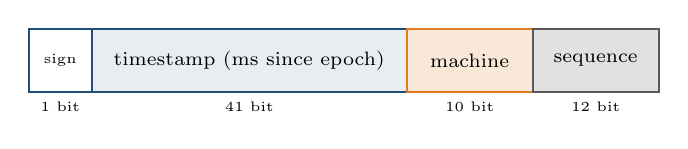
\begin{tikzpicture}[x=8mm,y=8mm]
  \draw[draw=cMain,thick] (0,0) rectangle (1,1);
    \node[font=\tiny] at (0.5,0.5) {sign};
    \node[font=\tiny,below] at (0.5,0)  {1 bit};
  \draw[draw=cMain,thick,fill=cMain!10] (1,0) rectangle (6,1);
    \node[font=\scriptsize] at (3.5,0.5) {timestamp (ms since epoch)};
    \node[font=\tiny,below] at (3.5,0)  {41 bit};
  \draw[draw=cAccent,thick,fill=cAccent!18] (6,0) rectangle (8,1);
    \node[font=\scriptsize] at (7,0.5) {machine};
    \node[font=\tiny,below] at (7,0)    {10 bit};
  \draw[draw=cGray,thick,fill=cGray!18] (8,0) rectangle (10,1);
    \node[font=\scriptsize] at (9,0.5) {sequence};
    \node[font=\tiny,below] at (9,0)    {12 bit};
\end{tikzpicture}
\vspace{4mm}
\begin{itemize}
  \item \textbf{41 bit 时间戳}：从 2024-01-01 起，可用 $\approx$ 69 年（到 2094 年）。
  \item \textbf{10 bit 机器位}：最多 1024 个进程，gomall 单实例够用。
  \item \textbf{12 bit 序列号}：单进程单毫秒最多 4096 个 ID = 单机峰值 4M/s ID 上限。
\end{itemize}
\srcnote{pkg/utils/snowflake/snowflake.go:11 epoch = 2024-01-01 UTC}
\end{frame}

\begin{frame}[fragile,shrink]{InitSnowflake：epoch 与机器位}
\begin{lstlisting}[language=Go,firstnumber=10,
  caption={\srcnote{pkg/utils/snowflake/snowflake.go:10--21}}]
func InitSnowflake(machineID int64) {
    snowflake.Epoch = time.Date(
        2024, 1, 1, 0, 0, 0, 0, time.UTC,
    ).UnixNano() / 1000000
    var err error
    node, err = snowflake.NewNode(machineID)
    if err != nil {
        panic(err)
    }
}

func GenSnowflakeID() int64 {
    return node.Generate().Int64()
}
\end{lstlisting}
\end{frame}

\begin{frame}[shrink]{逐行讲：为什么这 12 行很要紧}
\begin{description}\setlength{\itemsep}{0.4mm}
  \item[\texttt{Epoch=2024-01-01}] 把基准从 1970 平移到 2024，41 bit 时间空间从"剩 16 年"变"剩 69 年"。
  \item[\texttt{machineID}] 部署时由配置注入，多副本必须各不相同；冲突 = 双发出现\textbf{重复订单号} = 财务对账炸。
  \item[\texttt{NewNode 失败 panic}] 启动期就挂掉，比运行期偶发生成失败更安全 —— 订单号是金融语义，不能"先跑起来再说"。
  \item[\texttt{Generate().Int64()}] 一次返回 int64，方便存 \texttt{order.order\_num bigint unsigned}。
\end{description}
\vspace{2mm}
\keypoint{雪花是\textbf{本地无锁}的——OrderCreate 调用它零网络成本，\\
这是实测 50,319 RPS / p95 2.33ms 的硬前提。}
\srcnote{stressTest/REPORT.md \S 4 幂等下单 50K RPS / p95 2.33ms}
\end{frame}

% ============================================================
\section{库存预扣 vs 真扣：业务取舍}
% ============================================================

\begin{frame}[shrink]{30 分钟未付窗口：商家 vs 用户的拉扯}
\resizebox{0.95\textwidth}{!}{%
\begin{tikzpicture}[node distance=14mm and 16mm,font=\scriptsize]
  \node[node-box]                          (u) {用户加购};
  \node[node-box,right=of u,node-warn]     (c) {下单\\reserved += n};
  \node[node-box,right=of c,node-warn]     (w) {等待支付\\30 min 窗口};
  \node[node-box,right=of w,node-ok]       (p) {支付成功\\reserved $\to$ sold};
  \node[node-box,below=of c,node-warn]     (t) {超时未付\\reserved $\to$ available};
  \draw[arrow] (u) -- (c);
  \draw[arrow] (c) -- (w);
  \draw[arrow] (w) -- (p);
  \draw[arrow-alert] (w.south) -- (t.east);
\end{tikzpicture}}
\vspace{2mm}
\begin{tabular}{@{}p{0.45\linewidth}p{0.45\linewidth}@{}}
\toprule
\textbf{对商家不利} & \textbf{对用户有利} \\
\midrule
30 min 内库存被锁、不能转卖 & 下单时看到"还有 5 件"就一定还有 \\
峰值压货 = 现金流压力 & 不会"下完单告诉你没货了" \\
恶意占库（薅羊毛挂单）& 信任感建立 \\
\bottomrule
\end{tabular}
\vspace{1mm}
\keypoint{业务取舍：用 30 min "短期锁仓"换"下单不超卖"的承诺 —— 客户体验 > 商家短期周转。}
\srcnote{repository/cache/inventory.go:25--26 ErrStockInsufficient；internal/order/service.go:157--161 关单延迟：MQ 30min 主路径 + Cron 15min 兜底，详见 deck 07}
\end{frame}

\begin{frame}[shrink]{为什么不"下单即真扣"}
\begin{itemize}
  \item \textbf{方案 A：下单立即扣 sold} —— 用户取消 / 未支付 = 库存白损失，得回滚 sold 表 = 状态机更复杂。
  \item \textbf{方案 B：支付时才扣（不预扣）} —— 用户 A 拍下 $\to$ 用户 B 同时拍下 $\to$ 两人都付钱 $\to$ 超卖。
  \item \textbf{方案 C：gomall 选 = reserve 预扣 + commit 真扣两阶段}：
    \begin{itemize}
      \item 下单：\texttt{available -= n; reserved += n} —— 锁住但未消耗
      \item 支付：\texttt{reserved -= n} —— 真正售出
      \item 取消 / 超时：\texttt{reserved -= n; available += n} —— 完整退回
    \end{itemize}
\end{itemize}
\vspace{2mm}
\small \textbf{业务不变量}：\texttt{available + reserved + sold $\equiv$ 初始水位}，\\
任何一刻巡检脚本读三个桶相加 = 商品总库存 $\to$ 不平就告警。
\srcnote{repository/cache/inventory.go:32--66 reserve/commit/release 三脚 Lua；:78--125 Go 封装}
\end{frame}

% ============================================================
\section{下单是金融事件：三步必须原子}
% ============================================================

\begin{frame}[shrink]{OrderCreate 拆成三段}
\begin{tikzpicture}[node distance=10mm and 14mm]
  \node[node-box,node-warn] (r) {\textcolor{black}{1.Redis Reserve}\\available -= n\\reserved += n};
  \node[node-box,right=of r] (t) {\textcolor{black}{2.DB Transaction}\\INSERT order\\INSERT outbox};
  \node[node-box,right=of t,node-ok] (m) {\textcolor{black}{3.MQ delay}\\超时取消任务};
  \draw[arrow] (r) -- (t);
  \draw[arrow] (t) -- (m);
\end{tikzpicture}
\vspace{2mm}
\begin{itemize}
  \item \textbf{第 1 步}：Redis Lua 原子 reserve，失败 = \texttt{ErrStockInsufficient} 直接拒，不进 DB。
  \item \textbf{第 2 步}：同一 \texttt{gorm.Transaction} 写订单 + 写 outbox，二选一不行。
  \item \textbf{第 3 步}：投递延迟队列，超时未付款自动取消 $\to$ reserved 退回 available。
\end{itemize}
\srcnote{internal/order/service.go:55--171 全函数；internal/order/service.go:109--147 同事务写 order + 满减落账 + outbox}
\end{frame}

\begin{frame}[fragile,shrink]{OrderCreate 主体三步}
\begin{lstlisting}[language=Go,firstnumber=86,
  caption={\srcnote{internal/order/service.go:86--155 节选（满减计算/降级见 deck 13）}}]
order := &Order{
    UserID:    u.Id,
    ProductID: req.ProductID,
    Num:       int(req.Num),
    OrderNum:  uint64(snowflake.GenSnowflakeID()),
    // 满减落点 PromoRuleID / PromoDiscountCents / FinalCents 略
}

// 1) Redis 预扣库存（事务外）
if err = cache.ReserveStock(ctx, req.ProductID, int64(req.Num)); err != nil {
    return nil, err
}

// 2) 同事务写订单 + 应用满减 + 写 outbox
err = dao.NewDBClient(ctx).Transaction(func(tx *gorm.DB) error {
    if e := NewOrderDaoByDB(tx).CreateOrder(order); e != nil {
        return e
    }
    // s.promo.ApplyDiscountInTx(...) 预算耗尽降级为无折扣，略
    return outbox.NewOutboxDaoByDB(tx).Insert(
        "order", "OrderCreated", "order.created", order.ID,
        events.OrderCreated{ OrderID: order.ID, OrderNum: order.OrderNum,
            UserID: u.Id, ProductID: req.ProductID, Num: int(req.Num) })
})
if err != nil {
    // 3) 事务失败：把刚扣的预占库存放回
    _ = cache.ReleaseReservation(ctx, req.ProductID, int64(req.Num))
}
\end{lstlisting}
\end{frame}

\begin{frame}[shrink]{逐行讲：为什么 reserve 在 tx 外}
\begin{itemize}
  \item \textbf{Redis 不能加入 MySQL 事务}：跨存储两阶段提交业内基本不做，复杂度收益不划算。
  \item \textbf{reserve 失败必须早退}：库存不足 = 业务上 100\% 不可能成功，不该让 DB 也写一条又回滚。
  \item \textbf{tx 失败要补偿 release}：reserve 成功但 DB 失败 $\to$ 必须把扣的库存放回 available，否则\textbf{虚假占用}让其他用户也下不了单。
  \item \textbf{补偿不是事务的一部分}：即便 \texttt{ReleaseReservation} 也失败，DB 已 rollback，库存差额由对账兜底（\texttt{GetStockSnapshot} 巡检）。
\end{itemize}
\srcnote{repository/cache/inventory.go:78--125 reserve / commit / release 三脚}
\end{frame}

\begin{frame}[shrink]{逐行讲：为什么 outbox 必须在 tx 内}
\begin{itemize}
  \item 写订单 + 发 MQ 如果\textbf{拆成两步}：
  \begin{itemize}
    \item 写订单成功、发 MQ 前进程挂了 $\to$ \textbf{下游永远收不到 OrderCreated} $\to$ 不发货 $\to$ 客诉。
    \item 反过来：先发 MQ 再写 DB，DB 失败 $\to$ \textbf{幻影订单事件} $\to$ 发了不存在的货 $\to$ 商家亏。
  \end{itemize}
  \item \textbf{outbox 表充当桥梁}：写订单和写 outbox 用同一 \texttt{INSERT} 事务，要么都成功要么都没有。
  \item \textbf{异步 publisher} 扫 \texttt{status=pending} 的 outbox 行，发 MQ，发完更新成 \texttt{sent}。
  \item 这是 deck 11（Outbox 与一致性）在下单链路的落地。
\end{itemize}
\srcnote{internal/shared/outbox/repo.go:26--41 Insert 同 tx；internal/shared/outbox/publisher.go 扫表 publisher}
\end{frame}

\begin{frame}[shrink]{outbox 事件投递时序}
\resizebox{0.92\textwidth}{0.5\textheight}{%
\begin{tikzpicture}[node distance=10mm and 16mm,font=\scriptsize]
  \node[node-box,minimum width=26mm] (api) {API Goroutine};
  \node[node-box,below=of api,node-warn,minimum width=32mm] (tx)  {DB tx\\INSERT order\\INSERT outbox(pending)};
  \node[node-box,right=of tx,minimum width=26mm] (pub) {Publisher\\(扫 pending)};
  \node[node-box,right=of pub,node-ok,minimum width=22mm] (mq) {RabbitMQ};
  \draw[arrow] (api) -- (tx);
  \draw[arrow-async] (tx) -- node[above,font=\tiny,sloped]{异步扫表} (pub);
  \draw[arrow,transform canvas={yshift=2mm}] (pub) -- node[above,font=\tiny]{publish} (mq);
  \draw[arrow,transform canvas={yshift=-2mm}] (mq) -- node[below,font=\tiny]{ack $\to$ MarkSent} (pub);
\end{tikzpicture}}
\par\smallskip
{\small \textbf{业务侧好处}：API 返回时只承担一次 DB 写代价，用户感知延迟 < 5ms；MQ 发布失败由 publisher 重试，\textbf{不阻塞下单链路} = 不会因为 RMQ 抖一下整个下单挂掉。}
\srcnote{internal/shared/outbox/repo.go:44--79 FetchBatch + MarkSent + MarkFailed}
\end{frame}

% ============================================================
\section{幂等：755K 次请求 = 1 笔订单}
% ============================================================

\begin{frame}[shrink]{重复下单：用户狂点的真实场景}
\begin{itemize}
  \item \textbf{网络抖一下}：用户点"提交" $\to$ 转圈 $\to$ 没反应 $\to$ 再点一下 $\to$ 再点 $\to$ 连点 5 下。
  \item \textbf{双 11 客户端重试风暴}：APP 看到请求超时自动重试 3 次，1 次点击 = 4 次请求。
  \item \textbf{支付页双开}：用户在两个 tab 同时下单同一商品。
  \item \textbf{脚本党}：写脚本批量重试薅活动 —— 同一 token 打满请求。
\end{itemize}
\vspace{2mm}
\textbf{没有幂等会发生什么}：
\begin{itemize}
  \item 用户被\textbf{重复扣款} $\to$ 客服爆单 $\to$ 退款 $\to$ 信任崩塌。
  \item 库存被多次扣减 $\to$ 真实库存 = 5 但 reserved = 25 $\to$ 后来者全被拒。
  \item 商家看到 5 笔重复订单 $\to$ 不知道发不发货。
\end{itemize}
\srcnote{middleware/idempotency.go:35--112 Idempotency 中间件}
\end{frame}

\begin{frame}[shrink]{业务码 60002：客服一看就懂}
\begin{tabular}{@{}lll@{}}
\toprule
状态码 & 含义        & 客服话术 \\
\midrule
\texttt{50001}\,*  & 库存不足/上传异常  & "该商品已抢空，建议选购同款" \\
\texttt{60002}     & 幂等处理中        & "您的订单正在处理，请勿重复提交" \\
\texttt{20001}     & 商家鉴权失败      & "该店铺暂未营业" \\
\texttt{70001}     & 限流              & "当前访问拥挤，请稍后重试" \\
\texttt{70002}     & 熔断              & "下游服务异常，已为您保留请求" \\
\texttt{20008}     & 购物车重复加购    & "购物车已有该商品，已为您加件" \\
\bottomrule
\end{tabular}
\vspace{2mm}
\small *注：50001 是 \texttt{ErrorOss}（对象存储）；库存不足在代码里是 \texttt{cache.ErrStockInsufficient} 错误，业务码统一映射在 \texttt{pkg/e/code.go}。\\
\textbf{客户端硬约束}：HTTP 全是 200，必须按 \texttt{status} 字段分支，不能只看 HTTP code。
\srcnote{pkg/e/code.go:23--58 业务码 + middleware/idempotency.go:86--93 60002 返回路径}
\end{frame}

\begin{frame}[fragile,shrink]{Idempotency 中间件：状态机三态}
\begin{lstlisting}[language=Go,firstnumber=72,
  caption={\srcnote{middleware/idempotency.go:72--94 三态 switch}}]
switch state {
case 0:  // token 不存在
    c.JSON(http.StatusOK, gin.H{
        "status": e.ErrIdempotencyTokenInvalid,  // 60001
    })
    c.Abort()
    return
case 2:  // 已完成，回放上次响应体
    c.Header("X-Idempotent-Replay", "true")
    c.Data(http.StatusOK, "application/json; charset=utf-8",
        []byte(cached))
    c.Abort()
    return
case 3:  // 处理中，让客户端等
    c.JSON(http.StatusOK, gin.H{
        "status": e.ErrIdempotencyInProgress,    // 60002
    })
    c.Abort()
    return
}
// state == 1 抢到锁，c.Next() 真正执行业务
\end{lstlisting}
\end{frame}

\begin{frame}[shrink]{逐行讲：三态对应三种客户体验}
\begin{description}\setlength{\itemsep}{0.5mm}
  \item[\texttt{state=0}] token 过期 / 没传 $\to$ 让客户端\textbf{重新生成 key 再来} —— 防止陈年 token 重放攻击。
  \item[\texttt{state=2}] 已经成功过了 $\to$ \textbf{回放上次的 JSON} —— 用户看到的还是那笔订单号、同样的 money，体验上"我就下了一次"。
  \item[\texttt{state=3}] 还在处理中 $\to$ 返回 60002，前端\textbf{灰掉按钮}+ 500ms 后重试 —— 阻断"看似没反应就狂点"。
  \item[\texttt{state=1}] 抢到锁，真正下单 $\to$ \texttt{responseRecorder} 拷贝响应体 $\to$ 写回 done 态 $\to$ 下次重放就走 case 2。
\end{description}
\srcnote{middleware/idempotency.go:96--110 responseRecorder + CommitIdempotencyResult}
\end{frame}

\begin{frame}[shrink]{压测锚点：50,319 RPS / 755K 次 = 1 笔订单}
\begin{tabular}{@{}lrr@{}}
\toprule
场景 & 实测 & 备注 \\
\midrule
幂等下单 (\texttt{/orders/create}) RPS  & \textbf{50{,}319} & 50 VU × 15s \\
幂等下单 p95                            & 2.33 ms        & \\
幂等下单 max                            & 73 ms          & \\
\textbf{累计请求数}                     & 755{,}033      & 同一 Idempotency-Key \\
\textbf{实际写入 DB 的订单数}           & \textbf{1}     & 唯一一行 \\
\bottomrule
\end{tabular}
\vspace{3mm}
\small \textbf{业务意义}：同一 \texttt{Idempotency-Key} 重放 \textbf{75 万次}，DB 只多 1 行。\\
"重复下单防护"成本接近 0 —— 60002 直接读 Redis done 态。\\
order 表 6M 行 / 653 MB 不影响延迟 —— 不查表就不付代价。
\srcnote{stressTest/REPORT.md \S 4 幂等中间件 755{,}033 次 $\to$ 1 笔订单}
\end{frame}

% ============================================================
\section{同步下单 vs 异步下单}
% ============================================================

\begin{frame}[shrink]{两条下单路并存的业务理由}
\begin{tabular}{@{}lll@{}}
\toprule
路径 & 业务场景 & 用户体验 \\
\midrule
\texttt{/orders/create}  & 普通商品 / 流量平稳   & 一次请求拿到订单号 \\
\texttt{/orders/enqueue} & 秒杀 / 大促瞬时洪峰   & 拿 ticket，轮询 status \\
\bottomrule
\end{tabular}
\vspace{3mm}
\begin{itemize}
  \item \textbf{同步}：用户等响应的同时 DB 在写；DB 抖动 $\to$ 全部超时 $\to$ 转圈 $\to$ 流失。
  \item \textbf{异步}：MQ 顶住瞬时压力，consumer 平滑落库；代价 = 用户多一次轮询。
  \item \textbf{业务承诺}：P0 接口（下单 / 支付）\textbf{不挂限流}，靠异步削峰扛峰值（README SLO 行）。
\end{itemize}
\srcnote{internal/order/routes.go:12--14 两条路同挂 Idempotency；README.md \S 业务承诺 P0 不挂限流}
\end{frame}

\begin{frame}[shrink]{同步 vs 异步：链路对比}
\resizebox{0.95\textwidth}{!}{%
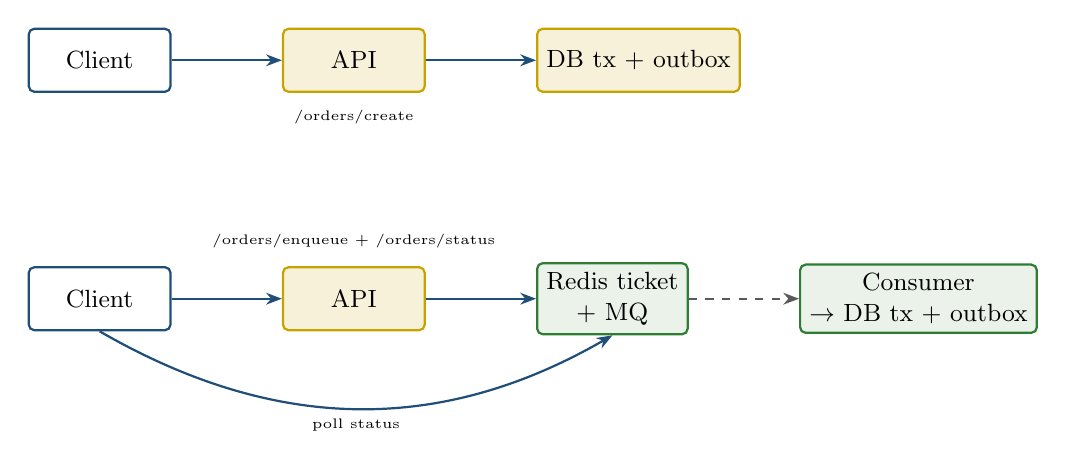
\begin{tikzpicture}[node distance=8mm and 14mm,font=\scriptsize]
  \node[node-box] (c1) {Client};
  \node[node-box,right=of c1,node-warn] (s1) {API};
  \node[node-box,right=of s1,node-warn] (d1) {DB tx + outbox};
  \draw[arrow] (c1) -- (s1);
  \draw[arrow] (s1) -- (d1);
  \node[font=\tiny,below=1mm of s1] {/orders/create};

  \node[node-box,below=22mm of c1] (c2) {Client};
  \node[node-box,right=of c2,node-warn] (s2) {API};
  \node[node-box,right=of s2,node-ok]   (q2) {Redis ticket\\+ MQ};
  \node[node-box,right=of q2,node-ok]   (w2) {Consumer\\$\to$ DB tx + outbox};
  \draw[arrow] (c2) -- (s2);
  \draw[arrow] (s2) -- (q2);
  \draw[arrow-async] (q2) -- (w2);
  \draw[arrow] (c2.south) to[out=-30,in=-150] node[below,font=\tiny]{poll status} (q2.south);
  \node[font=\tiny,above=1mm of s2] {/orders/enqueue + /orders/status};
\end{tikzpicture}}
\srcnote{internal/order/async.go:118--171 enqueue；:174--187 status}
\end{frame}

\begin{frame}[fragile,shrink]{OrderEnqueue 核心 12 行}
\begin{lstlisting}[language=Go,firstnumber=118,
  caption={\srcnote{internal/order/async.go:118--171 节选}}]
func (s *OrderSrv) OrderEnqueue(ctx context.Context,
    req *OrderCreateReq) (resp interface{}, err error) {

    if err = cache.ReserveStock(ctx,
        req.ProductID, int64(req.Num)); err != nil {
        return nil, err   // 库存不足直接拒
    }

    ticket := fmt.Sprintf("%d", snowflake.GenSnowflakeID())

    // 把 pending 状态写进 Redis，TTL 1h
    _ = defaultTicketStore.Put(ctx, ticket,
        OrderTicketStatus{Status: OrderTicketStatusPending},
        OrderTicketTTL)

    body, _ := json.Marshal(AsyncOrderTask{Ticket: ticket, ...})
    return OrderEnqueueResp{Ticket: ticket,
        Status: OrderTicketStatusPending},
        defaultAsyncProducer.Publish(ctx, body)
}
\end{lstlisting}
\end{frame}

\begin{frame}[shrink]{逐行讲：ticket 与 TTL 的业务取舍}
\begin{itemize}
  \item \textbf{ticket 用雪花生成}：和订单号同源，全局唯一、客户端无法伪造（防黑产构造假 ticket 查别人订单）。
  \item \textbf{TTL = 1h}：覆盖最长支付窗口 + 客服查单 + 一次客户端崩溃 —— 业务上"1 小时内一定有结论"。
  \item \textbf{ticket $\ne$ 订单号}：consumer 落库后回写 \texttt{OrderTicketStatus.OrderNum}，前端读 status 时一并拿到。
  \item \textbf{失败也写 ticket}：投递失败回写 \texttt{status=failed, reason=publish failed}，\textbf{前端不用纠结超时还是真失败} —— 一定能给用户一个明确答复。
\end{itemize}
\srcnote{internal/order/async.go:22--51 常量与状态结构；:163--166 失败写 failed}
\end{frame}

\begin{frame}[shrink]{ticket 状态机}
\centering
\resizebox{0.78\textwidth}{0.42\textheight}{%
\begin{tikzpicture}[node distance=10mm and 20mm,font=\scriptsize]
  \node[node-state,node-state-normal]              (p) {pending};
  \node[node-state,node-state-transition,above right=of p] (o) {ok\\+OrderNum};
  \node[node-state,node-state-alert,below right=of p]      (f) {failed\\+reason};
  \draw[arrow]       (p.north east) -- node[above=2pt,font=\tiny,sloped]{consumer 落库}    (o.west);
  \draw[arrow-alert] (p.south east) -- node[below=2pt,font=\tiny,sloped]{publish/db 失败} (f.west);
\end{tikzpicture}}
\vspace{2mm}
\begin{itemize}
  \item \textbf{pending}：API 已收单，consumer 未落库 —— 前端转圈但带文案"高峰排队中"。
  \item \textbf{ok}：DB 行已写，可走支付 —— 前端跳转支付页。
  \item \textbf{failed}：MQ 发布失败 / consumer 自检不通过 —— 前端弹"系统繁忙，请稍后重试"。
\end{itemize}
\srcnote{internal/order/async.go:25--27 三状态常量；:46--51 OrderTicketStatus 结构}
\end{frame}

\begin{frame}[shrink]{对账：reserve / commit / release 不变量}
\begin{itemize}
  \item 库存 Redis 双桶：\texttt{available + reserved + sold $\equiv$ 初始水位}。
  \item DB 订单 + outbox 同事务：两条记录要么都在要么都没有。
  \item ticket + DB 行：\texttt{OrderTicketStatus.Status=ok} $\iff$ \texttt{orders.order\_num} 存在。
\end{itemize}
\vspace{2mm}
任何一个不变量被破坏，巡检脚本应当告警：
\begin{itemize}
  \item Redis 双桶不平 $\to$ 库存对账脚本（\texttt{GetStockSnapshot}）$\to$ \textbf{客服报"我有 5 件但显示售罄"时第一时间查}。
  \item 订单与 outbox 数量不一致 $\to$ 直接 SQL JOIN 抽查 $\to$ \textbf{商家报"看不到这单"时第一时间查}。
  \item ticket=ok 但订单不存在 $\to$ consumer 写回路径异常 $\to$ \textbf{用户报"拍下了但订单页空"时第一时间查}。
\end{itemize}
\srcnote{repository/cache/inventory.go:128--138 GetStockSnapshot 巡检入口}
\end{frame}

% ============================================================
\section{深挖：epoch / 回拨 / 黑产 / 漏单}
% ============================================================

\begin{frame}[shrink]{为什么 epoch 选 2024-01-01 而不是 1970}
\begin{itemize}
  \item 标准 unix 时间戳 \texttt{1970-01-01} 到 2024 已经过去 $\approx$ 54 年 $\approx 1.7 \times 10^{12}$ ms。
  \item 41 bit 时间戳上限 $\approx 2.2 \times 10^{12}$ ms $\approx$ 69.7 年。
  \item 如果 epoch 用 1970：\textbf{剩余可用 $\approx$ 16 年}，2040 年雪花溢出 = 系统大故障。
  \item 如果 epoch 用 2024：\textbf{剩余可用 $\approx$ 69 年}，到 2094 年都不用动 = 业务寿命覆盖。
\end{itemize}
\vspace{2mm}
\begin{tikzpicture}[x=12mm,y=4mm]
  \draw[draw=cGray,thick] (0,0) -- (8,0);
  \foreach \x/\l in {0/1970,1.6/2024,4.5/2040,8/2094} {
    \draw[thick,draw=cMain] (\x,-0.4) -- (\x,0.4) node[above,font=\tiny]{\l};
  }
  \draw[draw=cAccent,thick,fill=cAccent!18] (1.6,-0.25) rectangle (8,0.25);
  \node[font=\tiny] at (4.8,0) {2024-epoch 可用 69 年};
\end{tikzpicture}
\srcnote{pkg/utils/snowflake/snowflake.go:11 epoch 常量；69 年是 41 bit 上限的精确计算}
\end{frame}

\begin{frame}[shrink]{时钟回拨：业内三种处理方式}
\begin{itemize}
  \item \textbf{阻塞等待}：检测到 \texttt{now < lastTimestamp} 时，sleep 到追上为止（gomall 用的库默认行为）。
  \item \textbf{扩展位补偿}：保留几个 bit 做"回拨计数器"，发生回拨时 +1，时间戳继续走（Twitter 原版）。
  \item \textbf{停机告警}：差距 > 阈值（如 5s）直接拒绝 ID 生成，让 SRE 介入（金融级）。
\end{itemize}
\vspace{2mm}
\begin{itemize}
  \item gomall 走第一种 —— \texttt{NewNode 失败 panic} 保证启动健康，运行期由库阻塞。
  \item 配合 NTP \texttt{slew} 模式（chronyd 默认）让时钟\textbf{平滑追赶}而不是跳变。
  \item 监控锚点：\texttt{GenSnowflakeID p99} —— 突然变大就是回拨告警的前哨。
\end{itemize}
\srcnote{pkg/utils/snowflake/snowflake.go:13--16 panic 策略；NTP slew vs step 由运维保证}
\end{frame}

\begin{frame}[shrink]{Redis / DB / outbox 三处失败的责任分摊}
\begin{tabular}{@{}lll@{}}
\toprule
失败点 & 表现 & 客服怎么解释 \\
\midrule
Redis reserve 失败 & 库存不足拒单    & "该商品已售罄" \\
DB INSERT order 失败 & gorm 报错     & "系统繁忙，请重试"+ 自动 release \\
DB INSERT outbox 失败 & 整 tx rollback & 同上 \\
publisher 发 MQ 失败 & outbox 留 pending & 用户看到订单，发货稍延后 \\
publisher 重试超限 & outbox 标 dead   & 客服联系商家手动补发货 \\
\bottomrule
\end{tabular}
\vspace{3mm}
\small \textbf{业务关键}：每一种失败都有\textbf{明确的归属者和兜底话术}，\\
没有"既不属于 A 也不属于 B"的灰区 —— 客服永远能给用户一个明确答复。
\srcnote{internal/shared/outbox/repo.go:62--79 MarkFailed 退避策略；internal/order/service.go:148--155 释放路径}
\end{frame}

\begin{frame}[shrink]{失败回滚状态机}
\begin{tikzpicture}[node distance=10mm and 16mm]
  \node[node-state,node-state-normal]                  (s0) {Start};
  \node[node-state,node-state-transition,right=of s0]  (rs) {Reserved};
  \node[node-state,node-state-normal,right=of rs]      (db) {DB OK\\+ Outbox};
  \node[node-state,node-state-normal,right=of db]      (sn) {Sent};
  \node[node-state,node-state-alert,below=of rs]       (rl) {Released};
  \node[node-state,node-state-alert,below=of sn]       (dd) {Dead};
  \draw[arrow]       (s0) -- node[above,font=\tiny]{ReserveOK} (rs);
  \draw[arrow]       (rs) -- node[above,font=\tiny]{tx commit} (db);
  \draw[arrow]       (db) -- node[above,font=\tiny]{publish ok}(sn);
  \draw[arrow-alert] (rs) -- node[left,font=\tiny]{tx fail}    (rl);
  \draw[arrow-alert] (db) -- node[right,font=\tiny]{超 max retry}(dd);
\end{tikzpicture}
\vspace{2mm}
\begin{itemize}
  \item \textbf{Released}：库存退回，订单不存在 —— 客户端可重试。
  \item \textbf{Dead}：订单存在但下游没收到 —— 用户能看到订单详情，发货 / 通知断 = 人工接管。
\end{itemize}
\srcnote{internal/shared/outbox/model.go OutboxStatusDead 终态；internal/shared/outbox/publisher.go 路径}
\end{frame}

\begin{frame}[shrink]{下单链路上的常见黑产手法}
\begin{itemize}
  \item \textbf{批量注册 + 单笔下单}：每个新号薅一次"新人券"，凑齐 100 单合并出货。
  \item \textbf{改 IP + 同设备}：脚本 + 代理池绕过单 IP 限流，但浏览器指纹一致。
  \item \textbf{地址聚合}：100 笔订单收件地址都是同一城中村 / 货代仓库。
  \item \textbf{支付聚合}：100 笔订单背后只有 2--3 张银行卡 / 同一个支付宝。
  \item \textbf{时间聚合}：凌晨 3:00--5:00 集中下单，避开运营值班。
\end{itemize}
\vspace{2mm}
\small \textbf{下单服务能给的钩子}：把 \texttt{ip / device\_id / address\_id / pay\_account} 作为事件字段写到 outbox，\\
异步推风控系统打分。下单链路本身\textbf{不做拦截判断}，否则尾延迟会被风控规则拖垮 = 违反 p99 < 500ms 业务承诺。
\srcnote{service/events/events.go:15--21 OrderCreated 已有 UserID/ProductID，扩展加风控字段}
\end{frame}

% ============================================================
\section{业务承诺与回顾}
% ============================================================

\begin{frame}[shrink]{下单链路的 SLO 业务承诺}
\begin{tabular}{@{}lll@{}}
\toprule
指标 & 业务承诺 & 实测对照 \\
\midrule
\texttt{/orders/create} p99 & < 500 ms          & p95 2.33 ms ✓ \\
可用率                       & 99.95\%（年宕 < 4h22min）& 单机本地实测 0\% 错 \\
峰值吞吐                     & 至少 50K RPS       & 50,319 RPS ✓ \\
基线对比（/ping）            & ——               & 64,254 RPS / p95 3.51ms \\
全链路 (/orders/list)        & ——               & 58,406 RPS / p95 5ms \\
重复请求 = 1 笔订单          & 强幂等            & 755K 次 = 1 笔 ✓ \\
\bottomrule
\end{tabular}
\vspace{2mm}
\keypoint{留 5--10× 余量给 GC / 网络抖动；P0 接口\textbf{不挂限流}，靠异步削峰扛峰值。}
\srcnote{stressTest/REPORT.md \S 各链路压测结果；README.md \S 业务承诺(SLO) 表}
\end{frame}

\begin{frame}[shrink]{把这条链拼回业务侧的一句话}
\begin{itemize}
  \item \textbf{购物车} = 凑单 / 比价 / 留存的中转，不是技术装饰。
  \item \textbf{地址} = 收货语义的快照，下单瞬间必须冻结。
  \item \textbf{雪花订单号} = 业务（防枚举 / 客服查单 / 商家对账）+ 性能（顺序写）的合谋。
  \item \textbf{库存预扣} = 用 30 min 短期锁仓换"下单不超卖"的承诺 —— 用户体验 > 商家短期周转。
  \item \textbf{OrderCreate 三步}：reserve 在事务外、outbox 在事务内、补偿在事务后。
  \item \textbf{幂等} = 755K 次请求 = 1 笔订单，重复防护成本 $\approx$ 0。
  \item \textbf{同步 / 异步两条路}：分别面对"平稳流量"和"瞬时洪峰"。
\end{itemize}
\vspace{2mm}
\keypoint{下单是金融事件 —— gomall 用"Redis 预扣 + DB 事务 + outbox 桥梁 + 幂等中间件"\\
把它拆成可证不变量、对每个角色都有交代的链路。}
\end{frame}

% ============================================================
\appendix
% ============================================================

\begin{frame}[shrink]{面试 Q\&A（1/2）}
\small
\textbf{Q1}：为什么 reserve 不放进 DB 事务？\\
\hspace{4mm}A：跨 Redis + MySQL 两阶段提交收益不抵复杂度。失败由 ReleaseReservation 补偿，对账兜底；业务上接受"极短时间窗"内库存差，因为有巡检脚本告警。
\vspace{1mm}

\textbf{Q2}：outbox 表写满了怎么办？\\
\hspace{4mm}A：publisher 周期归档 sent；dead 进单独表人工处理。归档脚本按月按 status 分区清；运维 SOP 写在告警手册里。
\vspace{1mm}

\textbf{Q3}：雪花时钟回拨在 gomall 怎么处理？\\
\hspace{4mm}A：库内部阻塞等待，NTP 用 slew 模式。监控 GenSnowflakeID p99 作为预警 —— 突然变大就是回拨前哨。
\vspace{1mm}

\textbf{Q4}：库存不足和幂等命中客户端怎么区分对待？\\
\hspace{4mm}A：库存不足 = \texttt{ErrStockInsufficient}（"已售罄"，终止重试）；幂等命中 = 60002（"处理中"，500ms 后重试）；done 态走 case 2 直接回放，前端用户感知"我就下了一次"。
\vspace{1mm}

\textbf{Q5}：755K 次请求 = 1 笔订单的业务价值？\\
\hspace{4mm}A：用户网络抖 / 双 11 客户端重试风暴 / 脚本党 $\to$ 不会重复扣款、不会重复占库存、商家不会看到 5 笔幽灵订单。
\end{frame}

\begin{frame}[shrink]{面试 Q\&A（2/2）}
\small
\textbf{Q6}：/orders/enqueue 比 /orders/create 多了什么风险？\\
\hspace{4mm}A：多一个 ticket 状态需要轮询；consumer 不可用时 ticket 一直 pending 需要 TTL 兜底；用户体验劣化（多一跳）。所以 1k QPS 别用异步，10k 必须，100k 配排队页。
\vspace{1mm}

\textbf{Q7}：30 分钟未支付窗口对商家不公平怎么办？\\
\hspace{4mm}A：业务取舍 —— 用户体验优先级 > 商家短期周转；窗口可配置（高单价商品调短到 15min，低单价拉长到 60min），通过 \texttt{repository/cache/inventory.go} 释放路径统一回收。
\vspace{1mm}

\textbf{Q8}：雪花 epoch 选 2024 之后想再改怎么办？\\
\hspace{4mm}A：不能动。同表里两种 epoch 解出的 ID 会撞，必须新表新字段或保持 epoch 永久不变。这是为什么 epoch 一开始就要选远（69 年覆盖业务寿命）。
\vspace{1mm}

\textbf{Q9}：100k QPS 营销活动，同步还是异步？\\
\hspace{4mm}A：异步 + 排队页 + 静默降级。同步路径留给 1k 量级的"普通下单"。P0 不挂限流 —— 削峰是把压力分散到时间轴上，不是拒绝用户。
\vspace{1mm}

\textbf{Q10}：批量注册薅券下单怎么拦？\\
\hspace{4mm}A：下单链路不拦（会拖垮 p99），把 ip/device/address/pay 写进 outbox 给风控异步判分；发货前二次决策 = 让风控决定要不要冻结订单。
\end{frame}

\begin{frame}[shrink]{代码位置一览}
\begin{description}\setlength{\itemsep}{0.2mm}
  \item[加购 / 地址]\srcnote{internal/cart/service.go:29--103；internal/address/service.go:25--124}
  \item[雪花生成]\srcnote{pkg/utils/snowflake/snowflake.go:10--25}
  \item[同步下单主体]\srcnote{internal/order/service.go:55--171 OrderCreate}
  \item[库存预扣/提交/释放]\srcnote{repository/cache/inventory.go:32--66 三脚 Lua；:78--125 Go 封装}
  \item[outbox 同事务写入 + 扫表]\srcnote{internal/shared/outbox/repo.go:26--79 Insert/FetchBatch/MarkSent/MarkFailed}
  \item[异步下单 + ticket 状态]\srcnote{internal/order/async.go:22--51 状态常量；:118--187 enqueue+status}
  \item[幂等中间件三态]\srcnote{middleware/idempotency.go:35--112}
  \item[业务码定义]\srcnote{pkg/e/code.go:23--58 20001/20008/60002/70001/70002}
  \item[OrderCreated 事件 / publisher]\srcnote{service/events/events.go:15--21；internal/shared/outbox/publisher.go}
  \item[路由]\srcnote{internal/order/routes.go:10--26；internal/cart/routes.go:8--17；internal/address/routes.go:8--17}
\end{description}
\vspace{1mm}
\keypoint{配套 deck：07 库存 / 08 营销 / 10 流量治理 / 11 一致性。}
\end{frame}

\end{document}
